\documentclass[tikz,border=8pt]{standalone}
\usepackage{ctex}
\usepackage{amsmath,amssymb}
\usetikzlibrary{arrows.meta,calc,angles,quotes,positioning,3d}
\definecolor{ink}{RGB}{31,43,57}
\definecolor{blue}{RGB}{35,91,166}
\definecolor{orange}{RGB}{224,111,20}
\definecolor{green}{RGB}{35,139,92}
\definecolor{red}{RGB}{190,52,52}
\tikzset{
 line cap=round,line join=round,
 body/.style={draw=ink,very thick},
 vec/.style={-{Latex[length=2.5mm]},draw=blue,very thick},
 force/.style={-{Latex[length=2.5mm]},draw=red,very thick},
 guide/.style={draw=ink!48,dashed},
 dim/.style={{Latex[length=2mm]}-{Latex[length=2mm]},draw=ink!70}
}
\begin{document}

% question-01：半球形洞与初始系绳几何
\begin{tikzpicture}[scale=.95]
 \fill[ink!5] (-4.8,-2.1)--(3.7,-3.0)--(5.0,1.1)--(-3.5,2.0)--cycle;
 \draw[body] (-4.8,-2.1)--(3.7,-3.0)--(5.0,1.1)--(-3.5,2.0)--cycle;
 \draw[body] (0,0) ellipse (3.0 and 1.20);
 \draw[ink!55,dashed,very thick] (-3,0) arc[start angle=180,end angle=360,x radius=3,y radius=1.2];
 \draw[blue!65,very thick] (-3,0) arc[start angle=180,end angle=360,x radius=3,y radius=2.8];
 \draw[blue!65,dashed,very thick] (-3,0) arc[start angle=180,end angle=0,x radius=3,y radius=.50];
 \coordinate (A) at (-2.45,.70);
 \coordinate (P) at (.38,1.18);
 \fill[orange] (A) circle(4pt) node[left] {$A$};
 \shade[ball color=orange!45] (P) circle(.25);
 \node[above=3pt] at (P) {$m$};
 \draw[red,very thick] (A)--(P) node[midway,above] {$L=R$};
 \coordinate (O) at (0,0);
 \fill[ink] (O) circle(2.5pt) node[below right] {$O$};
 \draw[guide] (O)--(P) node[midway,right] {$R$};
 \draw[vec] (-4.25,1.45)--++(0,-1.15) node[left] {$\boldsymbol g$};
 \node at (0,-3.65) {球在半球面与以 $A$ 为球心、半径 $R$ 的球面交线上运动};
\end{tikzpicture}

% solution-01：交圆几何与最低点受力
\begin{tikzpicture}[scale=.94]
 % 左：两个等半径球面的交圆。AO 垂直于交圆所在平面。
 \begin{scope}[xshift=-4.5cm]
  \coordinate (A1) at (-2.6,.35);
  \coordinate (C1) at (0,0);
  \coordinate (O1) at (2.6,-.35);
  \coordinate (B1) at (0,-2.45);
  \draw[blue,very thick] (C1) ellipse (.78 and 2.45);
  \draw[blue,dashed,very thick] (0,2.45) arc[start angle=90,end angle=270,x radius=.78,y radius=2.45];
  \draw[body] (A1)--(O1);
  \draw[body] (A1)--(B1) (O1)--(B1);
  \draw[guide] (C1)--(B1);
  \fill[ink] (A1) circle(3pt) node[left] {$A$};
  \fill[ink] (C1) circle(2.5pt) node[above=4pt] {$C$};
  \fill[ink] (O1) circle(3pt) node[right] {$O$};
  \shade[ball color=orange!45] (B1) circle(.20);
  \node[below=3pt] at (B1) {$B$};
  \node[above=5pt] at ($(A1)!0.5!(C1)$) {$R/2$};
  \node[below=5pt] at ($(C1)!0.5!(O1)$) {$R/2$};
  \node[right=4pt] at ($(C1)!0.58!(B1)$) {$\ell$};
  \node[align=center] at (0,-3.25) {交圆几何：$AC=CO=R/2$，$\ell=CB=\sqrt3R/2$};
 \end{scope}
 % 右：过 A、O、B 的截面，直接给出最低点的受力关系。
 \begin{scope}[xshift=4.4cm]
  \coordinate (A2) at (-2,0);
  \coordinate (C2) at (0,0);
  \coordinate (O2) at (2,0);
  \coordinate (B2) at (0,-3.464);
  \draw[body] (A2)--(O2) (A2)--(B2) (O2)--(B2);
  \draw[guide] (C2)--(B2);
  \fill[ink] (A2) circle(3pt) node[left] {$A$};
  \fill[ink] (C2) circle(2.5pt) node[above=3pt] {$C$};
  \fill[ink] (O2) circle(3pt) node[right] {$O$};
  \shade[ball color=orange!45] (B2) circle(.21);
  \node[below left=4pt] at (B2) {$B$};
  \node[left=4pt] at ($(A2)!0.23!(B2)$) {$R$};
  \node[right=4pt] at ($(O2)!0.23!(B2)$) {$R$};
  \draw pic[draw=blue,very thick,angle radius=7mm,"$30^\circ$" {xshift=-1mm,yshift=2mm}] {angle=C2--B2--A2};
  \draw pic[draw=blue,very thick,angle radius=7mm] {angle=O2--B2--C2};
  \draw[force] (B2)--($(B2)!0.42!(A2)$);
  \node[left=4pt] at ($(B2)!0.42!(A2)$) {$\boldsymbol T$};
  \draw[force] (B2)--($(B2)!0.42!(O2)$);
  \node[right=4pt] at ($(B2)!0.42!(O2)$) {$\boldsymbol N$};
  \draw[force] (B2)--++(0,-1.05) node[right=3pt] {$m\boldsymbol g$};
  \node[align=center] at (0,-5.05) {过 $A$、$O$、$B$ 的截面与最低点受力};
 \end{scope}
\end{tikzpicture}

% question-02：正三角形与正四面体初始构型
\begin{tikzpicture}[scale=.9]
 \begin{scope}[xshift=-4.2cm]
  \coordinate (A) at (0,2.0); \coordinate (B) at (-2.2,-1.4); \coordinate (D) at (2.2,-1.4);
  \fill[blue!7] (A)--(B)--(D)--cycle;
  \draw[body] (A)--(B)--(D)--cycle;
  \fill[orange] (A) circle(5pt) node[above] {$m_1$};
  \fill[orange] (B) circle(5pt) node[below left] {$m_2$};
  \fill[orange] (D) circle(5pt) node[below right] {$m_3$};
  \draw[dim] (B)+(0,-.55)--(D)+(0,-.55) node[midway,below] {$a$};
  \node at (0,-2.65) {正三角形};
 \end{scope}
 \begin{scope}[xshift=4.4cm]
  \coordinate (A) at (0,2.25); \coordinate (B) at (-2.2,-1.45); \coordinate (D) at (2.2,-1.45); \coordinate (E) at (.25,-.15);
  \fill[blue!6] (A)--(B)--(D)--cycle;
  \draw[body] (A)--(B)--(D)--cycle;
  \draw[body] (A)--(E) (B)--(E);
  \draw[guide,very thick] (D)--(E);
  \foreach \p/\lab/\pos in {A/m_1/above,B/m_2/below left,D/m_3/below right,E/m_4/right}{
   \fill[orange] (\p) circle(5pt) node[\pos] {$\lab$};
  }
  \node at (0,-2.65) {正四面体（虚线为背面棱）};
 \end{scope}
\end{tikzpicture}

% solution-02：以质心为缩放中心的相似坍缩
\begin{tikzpicture}[scale=.92]
 \coordinate (P1) at (0,2.35); \coordinate (P2) at (-2.7,-1.55); \coordinate (P3) at (2.7,-1.55);
 \coordinate (G) at (0,-.25);
 \draw[body] (P1)--(P2)--(P3)--cycle;
 \draw[guide] (P1)--(G) (P2)--(G) (P3)--(G);
 \foreach \p/\lab/\pos in {P1/m_1/above,P2/m_2/below left,P3/m_3/below right}{\fill[orange] (\p) circle(5pt) node[\pos] {$\lab$};}
 \fill[ink] (G) circle(3pt) node[right] {$G$};
 \draw[force] (P1)--($(P1)!0.42!(G)$) node[right] {$\boldsymbol F_1$};
 \draw[vec] (P2)--($(P2)!0.34!(G)$);
 \draw[vec] (P3)--($(P3)!0.34!(G)$);
 \draw[orange!70,very thick] ($(P1)!0.42!(G)$)--($(P2)!0.42!(G)$)--($(P3)!0.42!(G)$)--cycle;
 \node[align=center] at (5.0,.65) {$\boldsymbol r_i(t)=\lambda(t)\boldsymbol r_i(0)$,\\所有棱长同时缩放为 $a\lambda(t)$};
 \node[draw=ink!35,rounded corners,fill=white,align=center] at (0,-3.1)
 {$\displaystyle \ddot\lambda=-\frac{G\sum_i m_i}{a^3\lambda^2}$，\\三角形与四面体均保持相似};
\end{tikzpicture}

% question-03：卡诺热机、有限温差散热器与环境
\begin{tikzpicture}[scale=.92]
 \node[draw=red!75!black,very thick,rounded corners,fill=red!6,minimum width=2.25cm,minimum height=2.0cm] (hot) at (-4.5,0) {高温热源 $T_1$};
 \node[draw=ink,very thick,circle,fill=ink!5,minimum size=1.45cm] (eng) at (-1.2,0) {工质};
 \node[draw=blue,very thick,rounded corners,fill=blue!6,minimum width=2.25cm,minimum height=2.0cm] (cold) at (2.2,0) {低温热源 $T$};
 \node[draw=green!70!black,very thick,rounded corners,fill=green!6,minimum width=1.75cm,minimum height=2.0cm] (env) at (5.5,0) {环境 $T_2$};
 \draw[-{Latex[length=3mm]},red!75!black,very thick] (hot)--(eng) node[midway,above] {$\dot Q_1$};
 \draw[-{Latex[length=3mm]},blue,very thick] (eng)--(cold) node[midway,above] {$\dot Q_2$};
 \draw[-{Latex[length=3mm]},green!70!black,very thick] (cold)--(env) node[midway,above] {$\alpha(T-T_2)$};
 \draw[-{Latex[length=3mm]},orange,very thick] (eng)--++(0,-1.65) node[below] {$P$};
 \draw[ink!55,dashed,rounded corners] (-2.3,1.45) rectangle (3.35,-1.2);
 \node[ink!65] at (.55,1.72) {卡诺热机};
\end{tikzpicture}

% solution-03：功率关于低温热源温度的极值
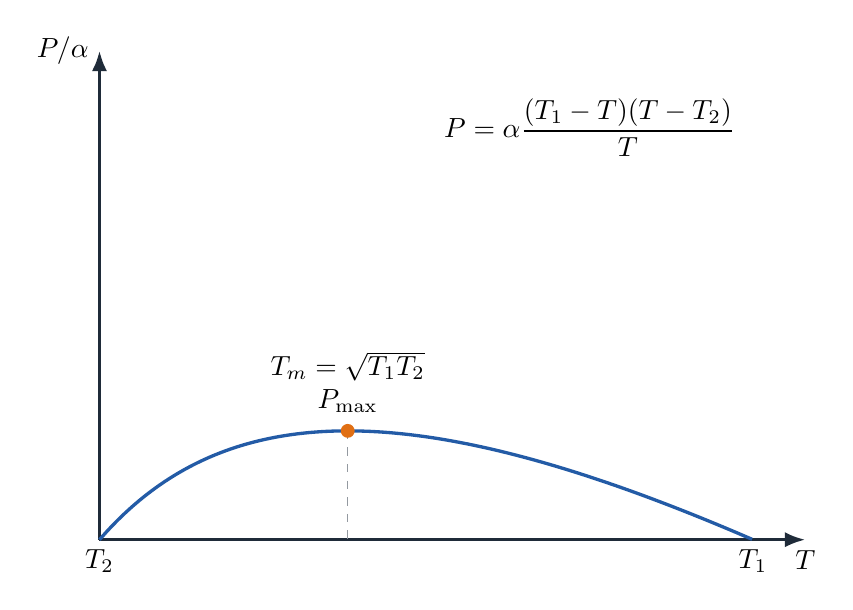
\begin{tikzpicture}[x=8.3cm,y=1.15cm]
 \draw[-{Latex[length=2.6mm]},body] (0,0)--(1.08,0) node[below] {$T$};
 \draw[-{Latex[length=2.6mm]},body] (0,0)--(0,5.4) node[left] {$P/\alpha$};
 \draw[blue,very thick,domain=0:1,samples=100,smooth]
  plot (\x,{5*(1-\x)*\x/(.6+\x)});
 \coordinate (M) at (.3798,{5*(1-.3798)*.3798/(.6+.3798)});
 \draw[guide] (M)--(.3798,0);
 \fill[orange] (M) circle(2.5pt);
 \node[above=3pt,align=center] at (M) {$T_m=\sqrt{T_1T_2}$\\$P_{\max}$};
 \node[below] at (0,0) {$T_2$};
 \node[below] at (1,0) {$T_1$};
 \node[align=left] at (.75,4.55)
 {$\displaystyle P=\alpha\frac{(T_1-T)(T-T_2)}{T}$};
\end{tikzpicture}

% question-04：两个相切玻璃球构成无焦系统
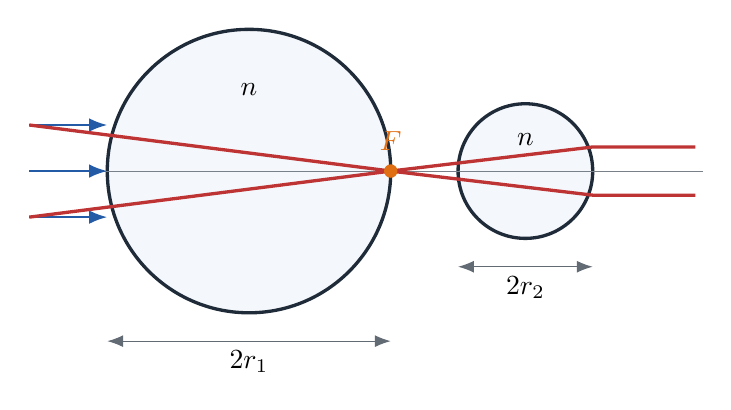
\begin{tikzpicture}[scale=.9]
 \coordinate (C1) at (-1.9,0); \coordinate (C2) at (2.0,0);
 \fill[blue!5] (C1) circle(2.0); \fill[blue!5] (C2) circle(.95);
 \draw[body] (C1) circle(2.0) (C2) circle(.95);
 \draw[ink!60] (-5,0)--(4.5,0);
 \foreach \yy in {-.65,0,.65}{
  \draw[-{Latex[length=2.3mm]},blue,thick] (-5,\yy)--(-3.9,\yy);
 }
 \draw[red,very thick] (-5,.65)--(.1,0)--(2.95,-.34)--(4.4,-.34);
 \draw[red,very thick] (-5,-.65)--(.1,0)--(2.95,.34)--(4.4,.34);
 \fill[orange] (.1,0) circle(2.7pt) node[above=4pt] {$F$};
 \draw[dim] (-3.9,-2.4)--(.1,-2.4) node[midway,below] {$2r_1$};
 \draw[dim] (1.05,-1.35)--(2.95,-1.35) node[midway,below] {$2r_2$};
 \node at (-1.9,1.15) {$n$}; \node at (2,.45) {$n$};
\end{tikzpicture}

% solution-04：有限物距时第一球成像与第二球移动
\begin{tikzpicture}[scale=.92]
 \draw[-{Latex[length=2.5mm]},ink!65] (-5.5,0)--(5.7,0);
 \coordinate (S) at (-5,0); \coordinate (C1) at (-1.5,0);
 \coordinate (I) at (1.7,0); \coordinate (C2) at (2.7,0);
 \fill[orange] (S) circle(3pt) node[below] {物点};
 \fill[blue!5] (C1) circle(1.35); \draw[body] (C1) circle(1.35);
 \fill[blue!5] (C2) circle(1.0); \draw[body] (C2) circle(1.0);
 \fill[red] (I) circle(2.6pt) node[above=5pt] {中间像 $I$};
 \draw[red,very thick] (S)--(-2.55,.82)--(I);
 \draw[red,very thick] (S)--(-2.55,-.82)--(I);
 \draw[red,very thick] (I)--(3.5,.62)--(5.3,.62);
 \draw[red,very thick] (I)--(3.5,-.62)--(5.3,-.62);
 \draw[dim] (S)+(0,-1.75)--(C1)+(0,-1.75) node[midway,below] {$u$};
 \draw[dim] (-.15,-1.75)--(I)+(0,-1.75) node[midway,below] {$\Delta=\dfrac{r_1^2}{u-r_1}$};
 \node[align=center] at (0,2.1) {$n=2$ 时第一球的后焦面、第二球的前焦面均在球面上};
\end{tikzpicture}

% question-05：圆柱、矩形线圈与三维磁场方向
\begin{tikzpicture}[scale=.9]
 \coordinate (F) at (-2.8,-.55); \coordinate (Rr) at (2.6,.75);
 \fill[ink!5] (-5,-2.2)--(3.8,-.6)--(5.1,2.1)--(-3.7,.55)--cycle;
 \draw[body] (-5,-2.2)--(3.8,-.6)--(5.1,2.1)--(-3.7,.55)--cycle;
 \draw[body] (F) ellipse (.62 and 1.35);
 \draw[body] (Rr) ellipse (.62 and 1.35);
 \draw[body] ($(F)+(0,1.35)$)--($(Rr)+(0,1.35)$);
 \draw[body] ($(F)+(0,-1.35)$)--($(Rr)+(0,-1.35)$);
 \coordinate (A) at (-3.42,-.55); \coordinate (B) at (-2.18,-.55);
 \coordinate (D) at (1.98,.75); \coordinate (C) at (3.22,.75);
 \draw[orange,very thick,-{Latex[length=2.3mm]}] (A)--(B)--(C)--(D)--(A);
 \foreach \p/\lab/\pos in {A/A/left,B/B/below,C/C/right,D/D/above}{\fill[orange] (\p) circle(2.5pt) node[\pos] {$\lab$};}
 \draw[guide] (F)--(Rr) node[midway,above] {圆柱轴};
 \foreach \yy in {-.1,.7,1.5}{\draw[vec] (4.0,\yy)--++(1.45,0);}
 \node[blue] at (4.75,1.95) {$\boldsymbol B_0$};
 \node at (0,-2.15) {线圈平面初始为水平面，$\boldsymbol B_0$ 与圆柱轴垂直};
\end{tikzpicture}

% solution-05：纯滚动受力、磁通与转角
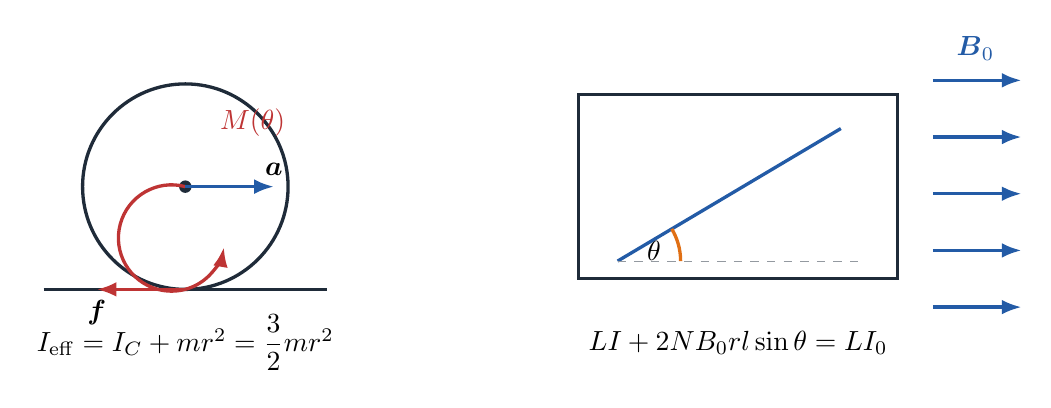
\begin{tikzpicture}[scale=.9]
 \begin{scope}[xshift=-4cm]
  \draw[body] (0,0) circle(1.45);
  \draw[body] (-2,-1.45)--(2,-1.45);
  \fill[ink] (0,0) circle(2.5pt);
  \draw[force] (0,0) arc[start angle=75,end angle=350,radius=.75];
  \node[red] at (.95,.9) {$M(\theta)$};
  \draw[force] (0,-1.45)--++(-1.25,0) node[below] {$\boldsymbol f$};
  \draw[vec] (0,0)--++(1.25,0) node[above] {$\boldsymbol a$};
  \node at (0,-2.2) {$I_{\rm eff}=I_C+mr^2=\dfrac32mr^2$};
 \end{scope}
 \begin{scope}[xshift=3.8cm]
  \coordinate (Q5A) at (-1.7,-1.05);
  \coordinate (Q5X) at (1.7,-1.05);
  \coordinate (Q5B) at (1.45,.82);
  \draw[body] (-2.25,-1.3) rectangle (2.25,1.3);
  \draw[blue,very thick] (Q5A)--(Q5B);
  \draw[guide] (Q5A)--(Q5X);
  \draw pic[draw=orange,very thick,angle radius=8mm,"$\theta$"] {angle=Q5X--Q5A--Q5B};
  \foreach \yy in {-1.7,-.9,-.1,.7,1.5}{\draw[vec] (2.75,\yy)--++(1.25,0);}
  \node[blue] at (3.35,1.95) {$\boldsymbol B_0$};
  \node[align=center] at (0,-2.2) {$LI+2NB_0rl\sin\theta=LI_0$};
 \end{scope}
\end{tikzpicture}

% question-06：两悬球与高内阻电源
\begin{tikzpicture}[scale=.95]
 \draw[body] (-3.2,2.5)--(3.2,2.5);
 \foreach \xx in {-3,-2.7,...,3}{\draw[ink!45] (\xx,2.5)--++(.25,.32);}
 \coordinate (P1) at (-1.25,2.5); \coordinate (P2) at (1.25,2.5);
 \coordinate (B1) at (-1.25,-1.3); \coordinate (B2) at (1.25,-1.3);
 \draw[body] (P1)--(B1) (P2)--(B2);
 \shade[ball color=blue!35] (B1) circle(.24); \shade[ball color=orange!45] (B2) circle(.24);
 \node[below] at (B1) {$-Q$}; \node[below] at (B2) {$+Q$};
 \draw[dim] (P1)+(0,.55)--(P2)+(0,.55) node[midway,above] {$d$};
 \draw[dim] (-2.0,2.5)--(-2.0,-1.3) node[midway,left] {$l$};
 \draw[ink,very thick] (P1)--(-1.25,3.35)--(-.55,3.35);
 \draw[ink,very thick] (P2)--(1.25,3.35)--(.55,3.35);
 \draw[ink,very thick] (-.55,3.1)--(-.55,3.6) (.55,2.95)--(.55,3.75);
 \node at (0,4.0) {$U$（内阻 $R$）};
 \draw[vec] (3.8,2.0)--++(0,-1.2) node[right] {$\boldsymbol g$};
\end{tikzpicture}

% solution-06：准静态平衡分支及失稳点
\begin{tikzpicture}[scale=.92]
 \begin{scope}[xshift=-3.8cm]
  \coordinate (P1) at (-1.5,2.2); \coordinate (P2) at (1.5,2.2);
  \coordinate (B1) at (-.75,-1.5); \coordinate (B2) at (.75,-1.5);
  \coordinate (V1) at (-1.5,-1.5);
  \draw[body] (P1)--(B1) (P2)--(B2);
  \draw[guide] (P1)--++(0,-3.7) (P2)--++(0,-3.7);
  \shade[ball color=blue!35] (B1) circle(.22); \shade[ball color=orange!45] (B2) circle(.22);
  \draw pic[draw=orange,very thick,angle radius=9mm,"$\theta$"] {angle=V1--P1--B1};
  \draw[dim] (B1)+(0,-.65)--(B2)+(0,-.65) node[midway,below] {$h=d-2l\sin\theta$};
  \draw[force] (B1)--++(.95,0) node[above] {$F_e$};
  \draw[force] (B1)--++(0,-1.0) node[left] {$mg$};
 \end{scope}
 \begin{scope}[xshift=3.1cm,x=5.2cm,y=1.0cm]
  \draw[-{Latex[length=2.5mm]},body] (0,0)--(1.1,0) node[below] {$\theta$};
  \draw[-{Latex[length=2.5mm]},body] (0,0)--(0,4.6) node[left] {$Q^2$};
  \draw[blue,very thick,domain=0:1,samples=80,smooth] plot (\x,{18*\x*(1-\x)^2});
  \coordinate (K) at (.333,{18*.333*(1-.333)^2});
  \fill[orange] (K) circle(2.5pt) node[above right] {临界点};
  \draw[guide] (K)--(.333,0);
  \node[align=left] at (.64,3.7) {$Q^2=4\pi\varepsilon_0mg$\\$\times(d-2l\sin\theta)^2\tan\theta$};
 \end{scope}
\end{tikzpicture}

% question-07：湖面几何与一个周期内的六条回波曲线
\begin{tikzpicture}[scale=.86]
 \begin{scope}[xshift=-4.7cm]
  \coordinate (O) at (0,0); \coordinate (A) at (-1.8,0); \coordinate (B) at (1.15,1.37);
  \draw[body] (O) circle(2.4);
  \draw[blue,dashed,very thick] (O) circle(1.8);
  \draw[body] (O)--(A) node[midway,below] {$x$};
  \draw[body] (O)--(B) node[midway,right] {$y$};
  \fill[orange] (A) circle(4pt) node[above left] {$A$};
  \fill[orange] (B) circle(4pt) node[above right] {$B$};
  \fill[ink] (O) circle(2.5pt) node[below] {$O$};
  \node at (0,-3.0) {圆形湖域与潜艇 $B$ 的运动轨道};
 \end{scope}
 \begin{scope}[xshift=1.0cm,x=6.4cm,y=1.25cm]
  \draw[-{Latex[length=2.4mm]},body] (0,0)--(1.08,0) node[below] {$t/T_B$};
  \draw[-{Latex[length=2.4mm]},body] (0,0)--(0,3.2) node[left] {$\Delta t/\mathrm s$};
  \foreach \x in {0,.25,.5,.75,1}{\draw[ink!35] (\x,0)--++(0,-.06);}
  \draw[red!70!black,very thick] (0,.333)--(1,.333) node[right] {1};
  \draw[green!70!black,very thick] (0,2.333)--(1,2.333) node[right] {2};
  \draw[ink!70,very thick] (0,2.667)--(1,2.667) node[right] {3};
  \draw[blue,very thick,domain=0:1,samples=80,smooth] plot (\x,{2*sin(180*\x)}) node[pos=.52,below] {4};
  \draw[orange,very thick,domain=0:1,samples=80,smooth] plot (\x,{2.333-2*\x+1.2*sin(180*\x)}) node[pos=.30,above] {5};
  \draw[violet,very thick,domain=0:1,samples=80,smooth] plot (\x,{.333+2*\x+1.2*sin(180*\x)}) node[pos=.70,above] {6};
  \node[left] at (0,.333) {$1/3$}; \node[left] at (0,2.333) {$7/3$}; \node[left] at (0,2.667) {$8/3$};
 \end{scope}
\end{tikzpicture}

% solution-07：六类回波路径的对应关系
\begin{tikzpicture}[scale=.93]
 \coordinate (O) at (0,0); \coordinate (A) at (-2.25,0); \coordinate (B) at (.9,1.65);
 \coordinate (L) at (-3.2,0); \coordinate (R) at (3.2,0);
 \coordinate (P) at (-.2,3.19); \coordinate (Q) at (2.65,-1.8);
 \draw[body] (O) circle(3.2);
 \draw[blue,dashed] (O) circle(2.25);
 \fill[orange] (A) circle(4pt) node[below left] {$A$}; \fill[orange] (B) circle(4pt) node[above right] {$B$};
 \fill[ink] (O) circle(2.5pt) node[below] {$O$};
 \foreach \p in {L,R,P,Q}{\fill[ink!65] (\p) circle(2.3pt);}
 \draw[red!70!black,very thick] (A)--(L)--(A);
 \draw[green!70!black,very thick] (A)--(R)--(A);
 \draw[ink!65,very thick] (A)--(L)--(R)--(A);
 \draw[blue,very thick] (A)--(B)--(A);
 \draw[orange,very thick] (A)--(P)--(B)--(A);
 \draw[violet,very thick] (A)--(Q)--(B)--(A);
 \node[align=left] at (5.1,.9)
 {\textcolor{red!70!black}{1}、\textcolor{green!70!black}{2}：一次湖壁反射\\
  \textcolor{ink!65}{3}：两次湖壁反射\\
  \textcolor{blue}{4}：在 $B$ 处一次反射\\
  \textcolor{orange}{5}、\textcolor{violet}{6}：湖壁与 $B$ 各反射一次};
\end{tikzpicture}

% question-08：流体本征系与运动参照系
\begin{tikzpicture}[scale=.92]
 \begin{scope}[xshift=-3.8cm]
  \draw[body,rounded corners,fill=blue!5] (-2.3,-1.5) rectangle (2.3,1.5);
  \foreach \p in {(-1.5,.7),(-.8,-.5),(0,1.0),(.7,-.9),(1.55,.25)}{\fill[orange] \p circle(3pt);}
  \foreach \yy in {-.85,-.25,.35,.95}{\draw[vec] (-1.7,\yy)--++(.7,0); \draw[vec] (1.7,\yy)--++(-.7,0);}
  \node at (0,2.0) {流体本征系 $S$：$g_x=0$，$T_{xx}=p$};
 \end{scope}
 \draw[-{Latex[length=3mm]},red,very thick] (-.8,0)--(.8,0) node[midway,above] {$u$};
 \begin{scope}[xshift=4.0cm]
  \draw[body,rounded corners,fill=red!4] (-2.3,-1.5) rectangle (2.3,1.5);
  \foreach \p in {(-1.5,.7),(-.8,-.5),(0,1.0),(.7,-.9),(1.55,.25)}{\fill[orange] \p circle(3pt); \draw[vec] \p--++(.65,0);}
  \node at (0,2.0) {运动系 $S'$：$e'$、$g'_x$、$T'_{xx}$};
 \end{scope}
\end{tikzpicture}

% solution-08：能量—动量张量在 x 方向的洛伦兹变换
\begin{tikzpicture}[scale=.95]
 \node[draw=ink!45,rounded corners,fill=blue!5,align=center,minimum width=4.2cm,minimum height=2.9cm] (rest) at (-4,0)
 {$\displaystyle T^{\mu\nu}=\begin{pmatrix}e&0\\[2pt]0&p\end{pmatrix}$\\本征系的 $t$--$x$ 子块};
 \node[draw=ink!45,rounded corners,fill=red!4,align=center,minimum width=5.0cm,minimum height=3.6cm] (move) at (4,0)
 {$\displaystyle e'=\gamma_u^2(e+\beta_u^2p)$\\[3pt]
  $\displaystyle g'_x=\gamma_u^2\frac{u}{c^2}(e+p)$\\[3pt]
  $\displaystyle T'_{xx}=\gamma_u^2(p+\beta_u^2e)$};
 \draw[-{Latex[length=3mm]},blue,very thick] (rest)--(move)
 node[midway,above,align=center] {沿 $x$ 方向变换\\$\beta_u=u/c$};
 \node[below=1.1cm of move,align=center] {$\displaystyle \gamma_u=\frac1{\sqrt{1-u^2/c^2}}$};
\end{tikzpicture}

\end{document}
